\part{Step Counter Algorithm}

    \chapter{Overview}

        This section covers the development and evaluation of the step counter algorithm. The algorithm aims to extract incidences of steps from the raw accelerometer data recorded on a smartphone. An example of raw accelerometer data of walking is shown below in Figure \ref{img_accel_ex}. It should be quite clear that the act of walking gives rise to periodic activity with a period corresponding to a single step. The act of walking is detailed in Naqvi, et. al. [CIT] and is as follows:

        \begin{enumerate}
            \item At the beginning of the step, the planted foot is pushed backwards into the floor.
            \item Static friction opposes this force. This provides the driving force forward.
            \item At the end of the step the stepping foot is placed on the floor and pushes forward into the floor.
            \item Again, static friction opposes this force, giving rise to a backwards force.
        \end{enumerate}

        \begin{figure}[h]
            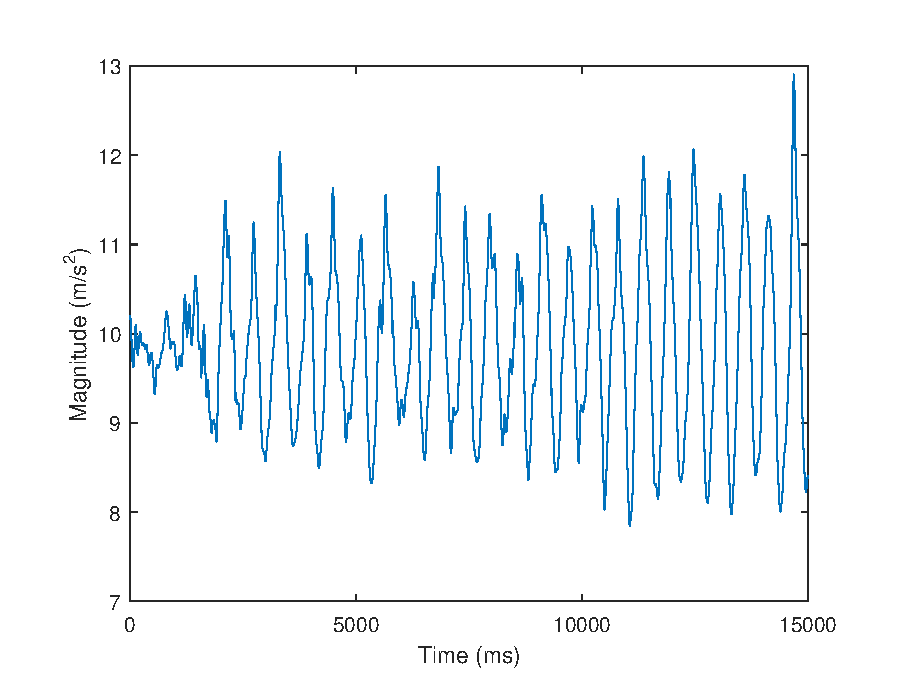
\includegraphics[width=\textwidth]{Images/accel_signal.eps}
            \centering
            \caption{Example of an accelerometer signal recorded during a period of walking.}
            \label{img_accel_ex}
        \end{figure}

        It is clear that each step will have both a peak and a trough associated with 2 and 4 respectively. The algorithm shall identify the peaks in the accelerometer signal. Effectively, the problem is one of peak detection in a noisy signal. 

        The algorithm is split into five stages, each responsible for a particular function. The data flows from stage to stage. All stages have an input data stream and output data stream, with the exception of the final stage which only has an input data stream. A block diagram is shown below in Figure \ref{img_sc_block}. Each one of the five stages will be described in detail in the following section.

        \begin{figure}[h]
            \includegraphics[width=\textwidth]{Images/step_counter_block.png}
            \centering
            \caption{Block diagram of the step counter algorithm.}
            \label{img_sc_block}
        \end{figure}

    \chapter{Algorithm Description}

        \section{Pre-Processing Stage}

            The Pre-Processing Stage is responsible for two functions:

            \begin{enumerate}
                \item Formatting the data received from the accelerometer into a usable format.
                \item Ensuring a constant sampling frequency by means of linear interpolation.
            \end{enumerate}

            The accelerometer data is received in the tri-axial format, however the algorithm is concerned with the magnitude rather than any single directional component because the the physical orientation of the device is unknown. The time stamps of the samples should also be scaled appropriately so that the first sample received from the user initiating the algorithm is at $t = 0$. The time stamps of the samples are provided in nanoseconds and are not given in standard UTC format, but as the time since system boot. The equations for these operations are simple and are as follows:

            \begin{equation}
                m = \sqrt{a_{x}^2 + a_{y}^2 + a_{z}^2},
            \end{equation}

            \begin{equation}
                t_{i,adjusted} = \frac{t_i - t_0}{t_s},
            \end{equation}

            where $m$ is the magnitude of the acceleration signal, $a_{x}$ is the acceleration in the x direction, $a_{y}$ is the acceleration in the y direction, $a_{z}$ is the acceleration in the z direction, $t_{i,adjusted}$ is the adjusted time stamp for the i-th sample, $t_i$ is the time stamp for the i-th sample, $t_0$ is the first time stamp in the trace, and $t_s$ is the time-scaling factor. For example, converting from nanoseconds to milliseconds, $t_s = 10^6$. 

            The data is then inserted into a simple data structure and is appended to an internal buffer of size 2. When this buffer is full, we will interpolate between these two points. The reason interpolation is needed is that although the developer can specific a desired sample rate in the Android application, there is no guarantee that the accelerometer will be sampled at this rate. An example of this is shown below in Figure \ref{img_sampling_freq} where time between samples is plotted against samples. For the filtering stage, we need to ensure that the data is sampled at a constant rate.

            The algorithm knows what the desired sample rate is, and will interpolate at this value. For example, if the sample rate is set to $f = 100 Hz$, then the algorithm will interpolate around $t = 0, 10, 20, 30, ... ms$. Each interpolated point is appended to the end of the stage's output data stream. The pseudocode for the linear interpolation is shown below.

            The equation for linear interpolation is as follows:

            \begin{equation}
                value = \frac{y_1 - y_0}{t_1 - t_0} t_{int} + y_0,
            \end{equation}

            where the two points that are being interpolated between are given by: $(t_1, y_1)$ and $(t_0, y_0)$, and the time to be interpolated at is given by $t_{int}$.

            \begin{figure}[h]
                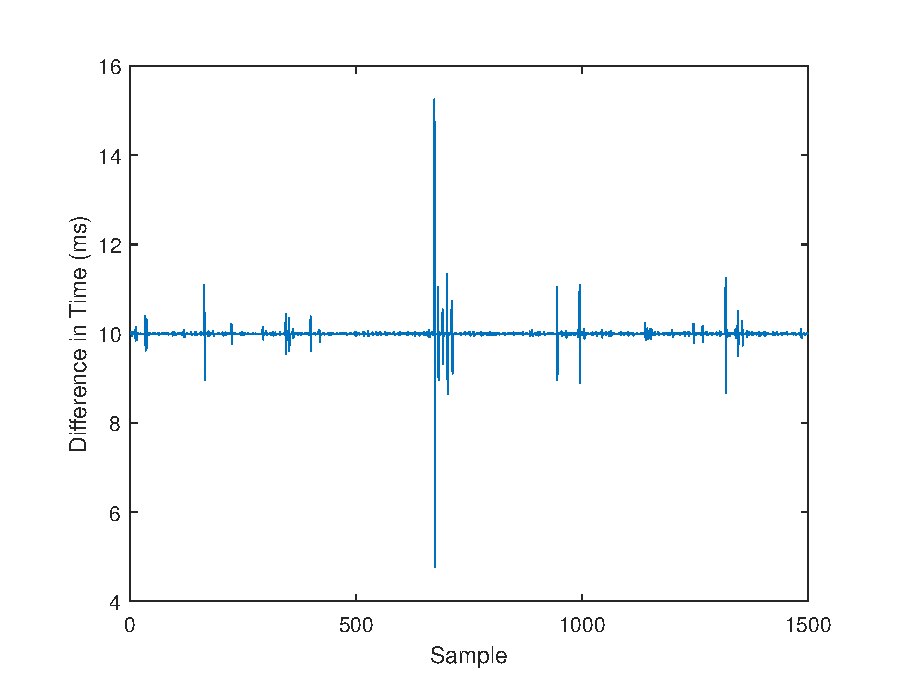
\includegraphics[width=\textwidth]{Images/sampling_freq.eps}
                \centering
                \caption{Time differences between samples for a 100Hz sampled signal. Note that the non-constant sampling times leads to the requirement for interpolation.}
                \label{img_sampling_freq}
            \end{figure}

        \section{Filtering Stage}

            The function of the filtering stage is to smooth the signal by removing as much of the high frequency noise from the acceleromater as possible.

            The filter required is a simple finite impulse response (FIR), low-pass digital filter. Ideally, this would be a steep-low pass filter with a frequency response described by Figure \ref{img_ideal_filter} below. However, this is impossible to achieve due to the infinite impulse response in the time domain (top-hat transforms to the sinc function). In order to capture the a variety of walking speeds, the cutoff of these filters will aim to be around 3 Hz. This should be sufficient to capture the walking of even the speediest walkers, as this would translate to an pace of $5.4 mph$ according to the ratio of $2000 steps = 1 mile$ as given by the American College of Sports Medicine [CIT]. Note that the average walking pace was found to be $3.1 mph$ in a study by Knoblauch, et. al. [CIT].

            An example of the prefiltered signal and the filtered signal is shown below in Figure \ref{img_filtered_signal}.

            \begin{figure}[h]
                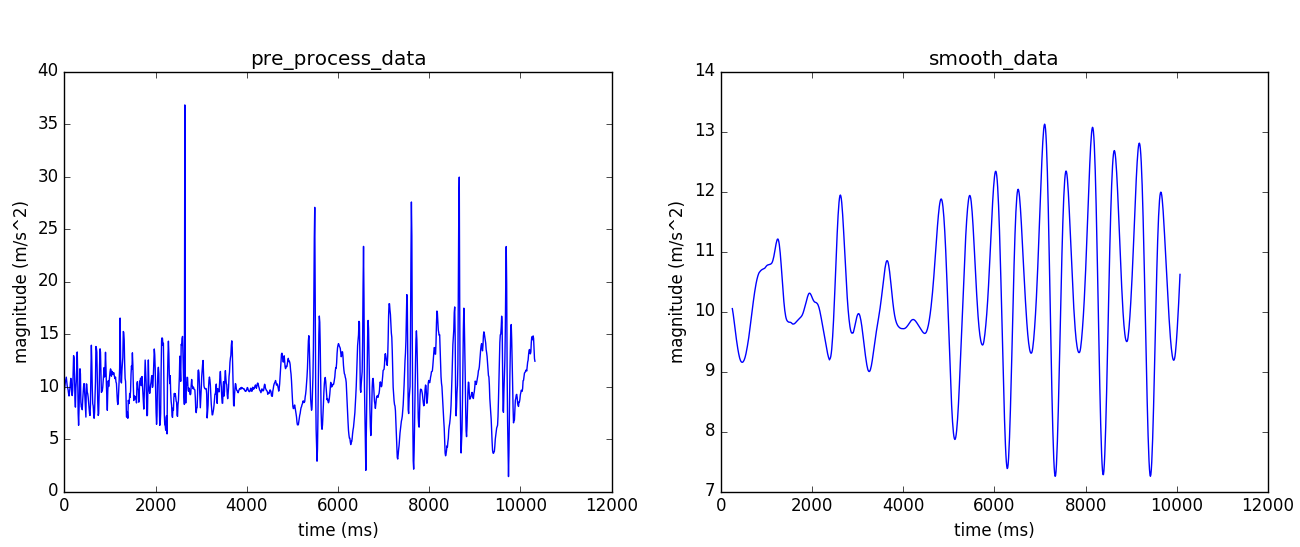
\includegraphics[width=\textwidth]{Images/filtered_signal.png}
                \centering
                \caption{Example of a signal being filtered. Filter used: Gaussian Filter with $N=51$ and $\sigma=0.35$. Note the large peaks due to noise are filtered out entirely.}
                \label{img_filtered_signal}
            \end{figure}

            A few filters were implemented for performance testing.

            \subsection{Moving Average}

                This is a very simple filter, each point in the filter window are weighted equally such that:

                \begin{equation}
                    m_k = \frac{1}{N},
                \end{equation}

                where $m_k$ is the $k^{th}$ filter coefficient, and $N$ is the length of the filter. The frequency response of this filter is shown below in Figure \ref{img_cm_filter}.

                \begin{figure}[!th]
                    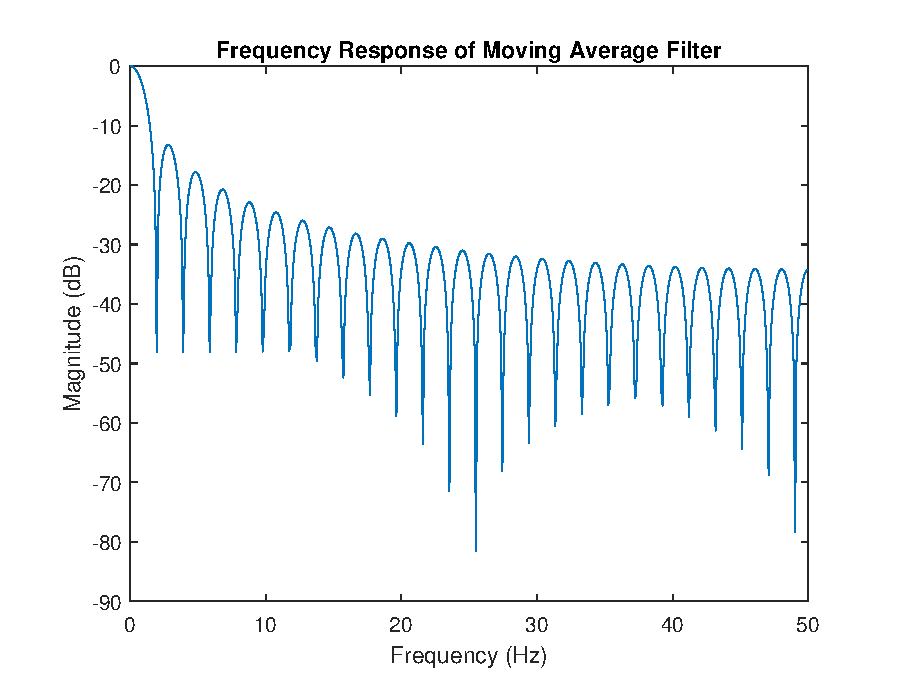
\includegraphics[width=\textwidth]{Images/cm_filter.eps}
                    \centering
                    \caption{Frequency response of the moving average filter with $N=31$.}
                    \label{img_cm_filter}
                \end{figure}

            \subsection{Gaussian Filter}

                This is a more complex filter, using a Gaussian as the waveform for the filter coefficients. This filter attempts to suppress the sidelobes of the center moving average filter by having a smoother transition to 0 magnitude. The weights of the filter are given by:

                \begin{equation}
                    g_k = \exp(-\frac{1}{2}(\frac{k - \frac{N-1}{2}}{\sigma \frac{N-1}{2}})^2),
                \end{equation}

                where $g_k$ is the $k^{th}$ coefficient of the filter, $N$ is the length of the filter window, and $\sigma$ is a parameter defining the standard deviation of the Gaussian. Note that the standard deviation also scales with the length of the filter. The frequency response of this filter is shown below in Figure \ref{img_ga_filter}.

                \begin{figure}[!th]
                    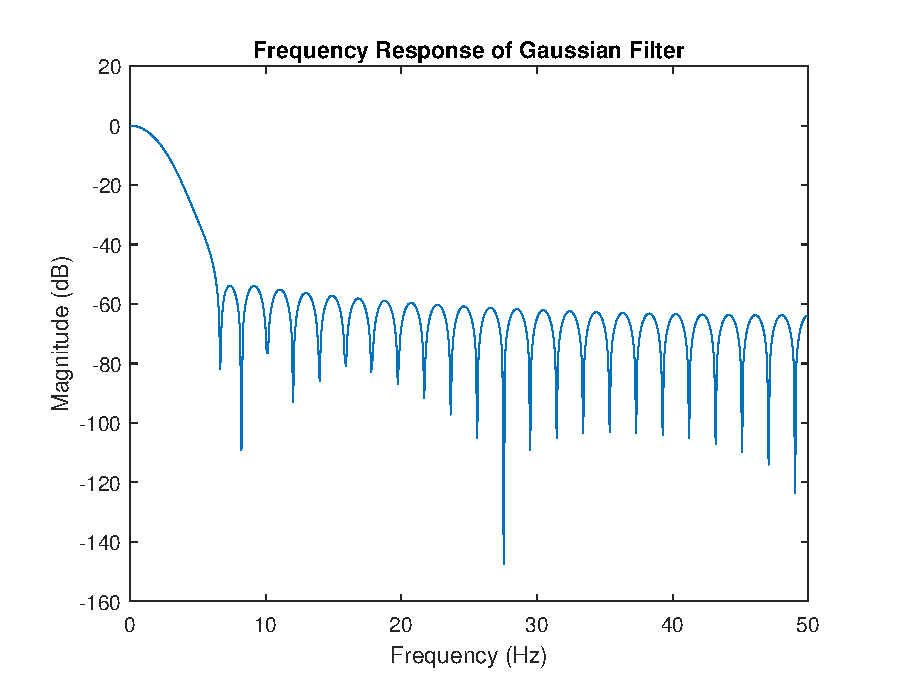
\includegraphics[width=\textwidth]{Images/ga_filter.eps}
                    \centering
                    \caption{Frequency response of the Gaussian filter with $N=51$ and $\sigma = 0.35$.}
                    \label{img_ga_filter}
                \end{figure}

            \subsection{Hann Filter}

                This is a similar filter to that of the Gaussian, where it attempts to smooth out the response by suppressing the sidelobes of the center moving average filter. The weights of the filter are derived from the Hann window [CIT] and are as follows: 

                \begin{equation}
                    h_k = \frac{1}{2}(1 - \cos(\frac{2\pi k}{N - 1}))
                \end{equation}

                where $h_k$ is the $k^{th}$ filter coefficient and $N$ is the length of the filter window. The frequency response of this filter is shown below in Figure \ref{img_ha_filter}.

                \begin{figure}[!th]
                    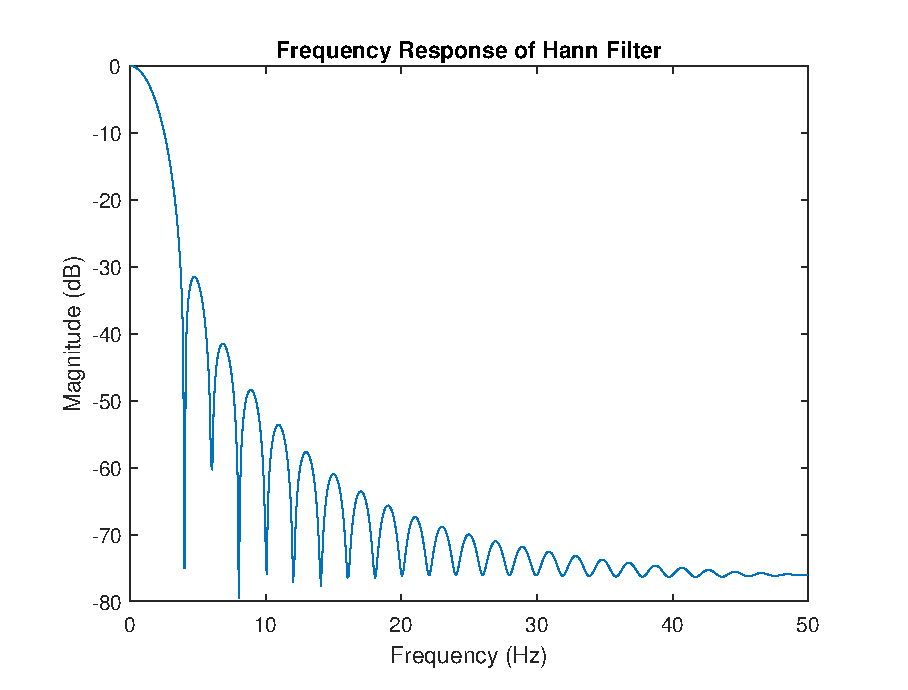
\includegraphics[width=\textwidth]{Images/ha_filter.eps}
                    \centering
                    \caption{Frequency response of the Hann filter with $N=51$.}
                    \label{img_ha_filter}
                \end{figure}  

            \subsection{Kaiser-Bessel Filter}

                This is the most complex filter design, designed by Kaiser [CIT] in order to achieve the desired attenutation at the cutoff frequency. It combines the ideal filter response (note a sinc function in the time domain) and a Bessel window to achieve the result. The calculation of the coeffcients are as follows.

                First, calculate the window shape parameter $\alpha$. 

                \begin{equation}
                    \alpha = 
                        \begin{cases}
                            0.1102(A - 8.7) & A \ge 50 \\
                            0.5842(A-21)^{0.4} + 0.07886(A-21) & 21 \leq A \geq 50 \\
                            0 & A \le 21
                        \end{cases},
                \end{equation}

                where $A$ is the desired attenuation at the cutoff frequency.

                Then calculate the coefficients of the Kaiser-Bessel window:

                \begin{equation}
                w_k = \frac{I_0(\alpha \sqrt{1 - (\frac{k - N_p}{N_p})^2})}{I_0(\alpha)},
                \end{equation}

                where $w_k$ is the $k^{th}$ coefficient of the window, $\alpha$ is the window shape parameter, $N_p$ is the midpoint of the filter, $N_p = \frac{N-1}{2}$ where $N$ is the length of the filter, and $I_0$ is the $0^{th}$ order Bessel function of the first kind.

                Then calculate the coefficients of the ideal filter response:

                \begin{equation}
                i_k = \frac{\sin(2\pi k\frac{F_c}{F_s})}{\pi k},
                \end{equation}

                where $i_k$ is the $k^{th}$ coefficient of the ideal filter response, $F_c$ is the desired cutoff frequency and $F_s$ is the sampling frequency.

                Finally, compute the coefficients of the filter with: 

                \begin{equation}
                b_k = w_ki_k,
                \end{equation}

                where $b_k$ is the $k^{th}$ coefficient of the Kaiser-Bessel filter response. The frequency response of this filter is shown below in Figure \ref{img_kb_filter}.

                \begin{figure}[!th]
                    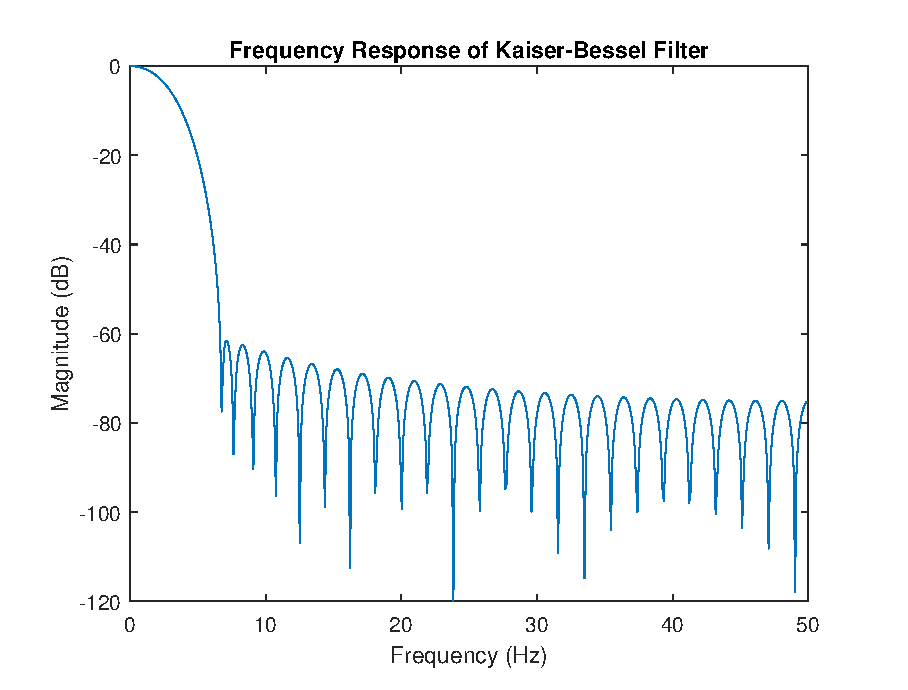
\includegraphics[width=\textwidth]{Images/kb_filter.eps}
                    \centering
                    \caption{Frequency response of the Kaiser-Bessel filter with $N=51$, $A=60dB$, $F_c = 3Hz$, and $F_s= 100Hz$.}
                    \label{img_kb_filter}
                \end{figure}  

        \section{Scoring Stage}

            The function of the scoring stage is to evaluate how 'peaky' any given point is. The result of this stage should increase the the magnitude of peak points, making them more obvious to a peak detector.

            A few methods were developed to be used in testing. These are detailed below.

            \subsection{Maximum Difference}

                This method uses the local neighbors of the point in question to determine how peaky the point is. It will look $N$ points to the left and determines the maximum difference between the point in question and those points. It will do the same for the $N$ points to the right, and then average the two maximum differences as the result.

                This operation will result in exaggerating peaks corresponding to steps as the following trough will cause a higher magnitude relative to peaks corresponding to other causes. An example of the output from a filtered signal to the scored signal using Maximum Difference is shown below in Figure \ref{max_diff_score}

                \begin{equation}
                x = \frac{\max\limits_k{(x_i - x_{i-k})} + \max\limits_k{(x_i - x_{i+k})}}{2},
                \end{equation}

                where $i$ is the point under consideration, and $x_n$ is the value of the signal at the $n^{th}$ sample.

                \begin{figure}[!th]
                    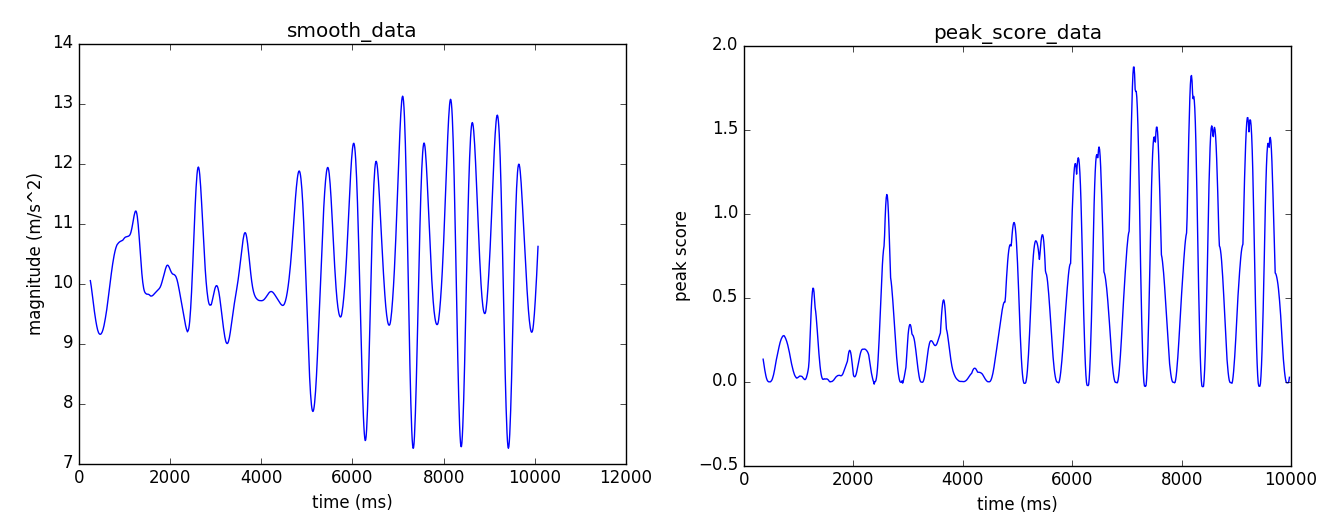
\includegraphics[width=\textwidth]{Images/max_diff_score.png}
                    \centering
                    \caption{Peak Scoring using Maximum Difference with $N=6$. Filtered data is on the left, smoothed data is on the right. Note how the large peaks are amplified, while the smaller ones are suppressed.}
                    \label{max_diff_score}
                \end{figure}                 

            \subsection{Mean Difference}

                This method is similar to Maximum Difference, except that instead of taking the maximum of the difference to the left and the right, Mean Difference takes the mean of all the differences. The effect is similar to Maximum Difference, but smaller in magnitude. It also preserves the overall shape of the waveform.

                An example of the output from a filtered signal to the scored signal using Mean Difference is shown below in Figure \ref{mean_diff_score}.

                \begin{equation}
                x = \frac{\sum_{k=-N, k\neq i}^{N} (x_i - x_{i+k})}{2N},
                \end{equation}

                where $i$ is the point under consideration and $N$ is the characteristic length of the Mean Difference operation.

                \begin{figure}[!th]
                    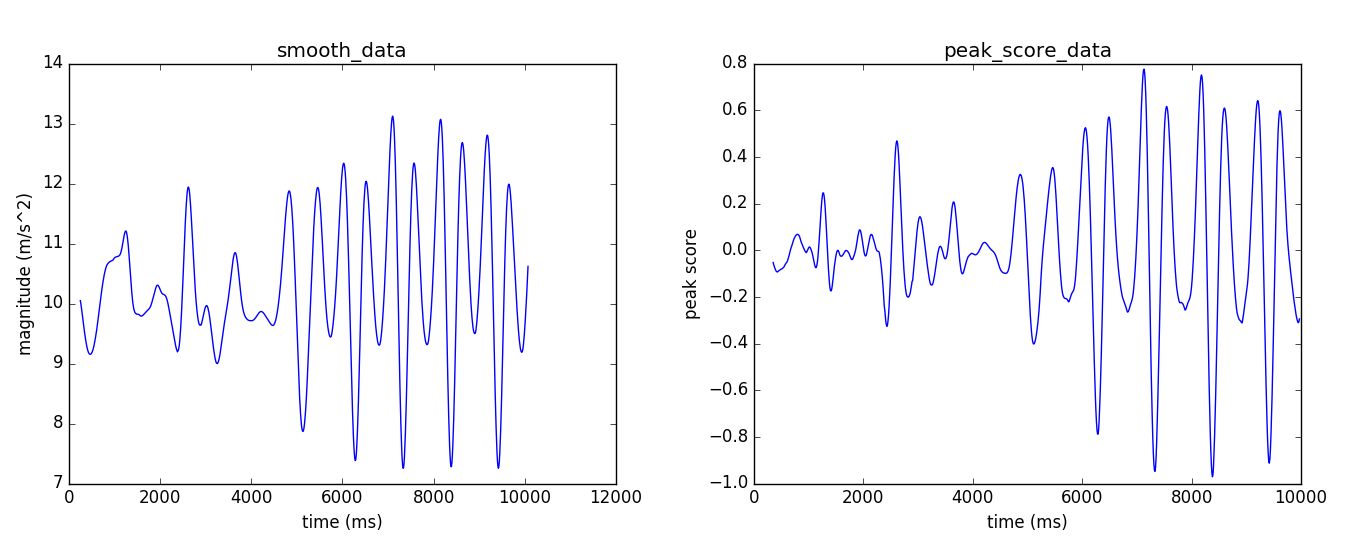
\includegraphics[width=\textwidth]{Images/mean_diff_score.png}
                    \centering
                    \caption{Peak Scoring using Mean Difference with $N=10$. Filtered data is on the left, scored data is on the right.}
                    \label{mean_diff_score}
                \end{figure}

            \subsection{Modified Pan-Tompkins Scoring}

                This method is a derivative from the famous algorithm by Pan and Tompkins [CIT] that was used for peak detection. 

                The original algorithm had four main steps: digital bandpass filter, differentiate the signal, square the signal, then a moving integration window to reconstitute the signal.

                From this baseline, a modified algorithm was developed:

                \begin{itemize}
                    \item Locally zero-mean the data around with a window of size $N$.
                    \item Set all the data points that are less than 0 to zero.
                    \item Square the data to amplify any large peaks.
                \end{itemize}

                The first step is integral as it ensures that when the data is squared, only truly large peaks get amplified. The second step is important to ensure that only positive peaks get detected. Without this, the algorithm would detect both the peak and trough.

                An example of this scoring using this method is shown below in Figure \ref{pan_tompkins_score}.

                \begin{figure}[!th]
                    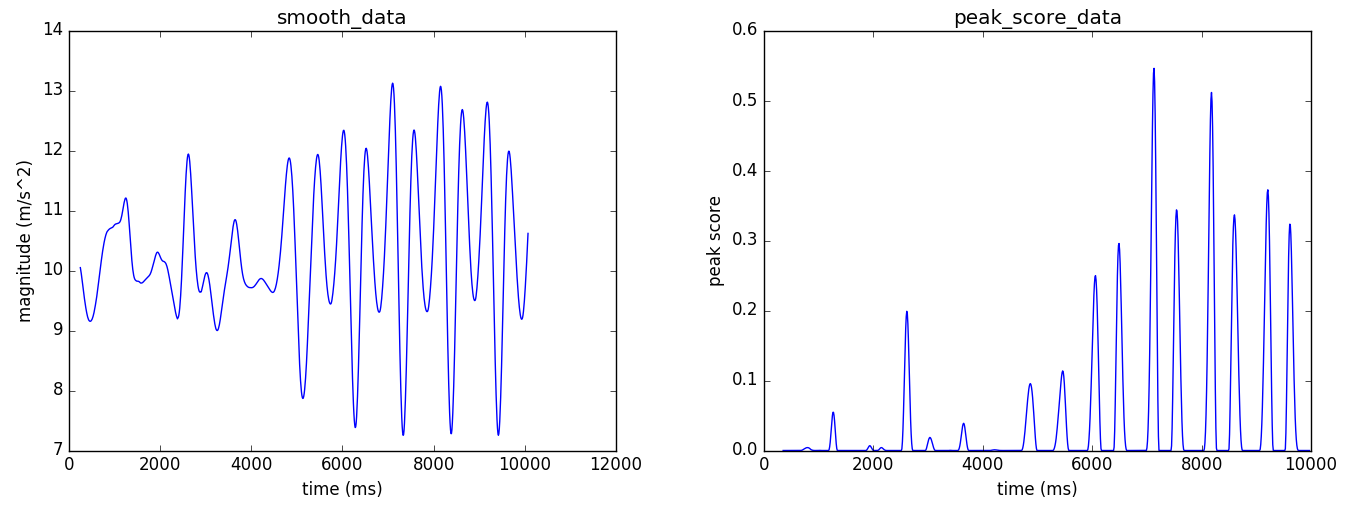
\includegraphics[width=\textwidth]{Images/pan_tompkins_score.png}
                    \centering
                    \caption{Peak Scoring using Modified Pan-Tompkins with $N=10$. Filtered data is on the left, scored data is on the right.}
                    \label{pan_tompkins_score}
                \end{figure}


        \section{Detection Stage}

        \section{Post-Processing Stage}

    \chapter{Data Collection Apparatus}

    \chapter{Algorithm Optimization}

    \chapter{Results}

    \chapter{Further Work}